\subsection{Experimentación inicial}

Como primera aproximación para reducir la cantidad de atributos utilizamos los algoritmos \textbf{SelectKBest} y \textbf{SelectPercentile} de
la sklearn.feature\_selection. La función de \( score \) elegida para ambos algoritmos fue \( chi2 \) (ya que era la 
utilizada por muchos ejemplos de la documentación de sklearn), y los features utilizados para la
experimentación fueron los Word Bags, tanto del body como del subject de los mensajes.

Luego de aplicar los algoritmos de reducción, utilizamos el modelo Bernoulli (Naive Bayes) como estimador para obtener el \( accuracy \) resultante
de la transformación de los datos.

\textbf{SelectKBest} toma un parámetro \( k \) que determina la cantidad de atributos a los cuales ajustarse.
\textbf{SelectPercentile} toma un parámetro \( p \) que determina un porcentaje de atributos a los cuales ajustarse.

A continuación se muestran los resultados obtenidos:

\begin{figure}
	\centerline{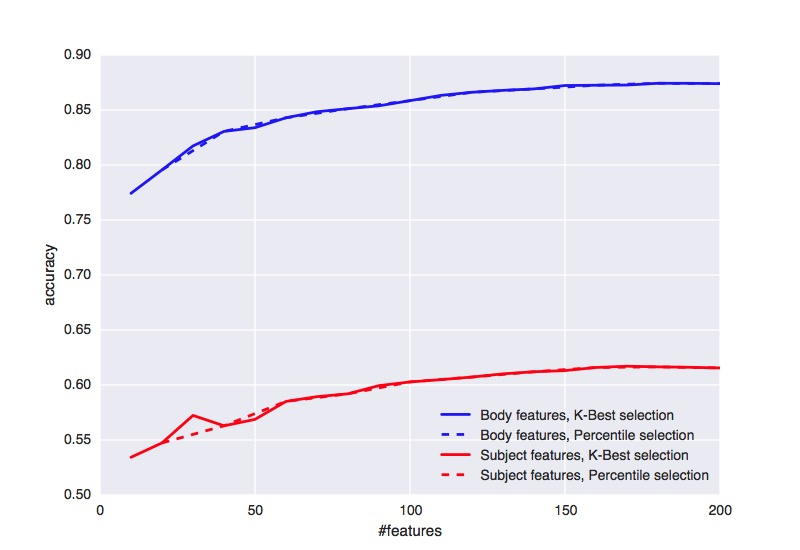
\includegraphics[scale=0.4]{figures/bernoulli_reduced_dimensionality.jpg}}
	\caption{Accuracy en función de cantidad de features resultante}
\end{figure}

La observación inmediata es que ninguno de los 2 algoritmos logra incrementar el accuracy al reducir la cantidad de atributos. De hecho, el accuracy máximo
se alcanza cuando el estimador utiliza la totalidad de los features. Es decir, no se produce reducción alguna.

Una segunda observación es que ambos algoritmos tienen una performance muy similar, si bien KBest parece dar un mejor resultado con una cantidad
de features menor.

Además, probamos reducir la cantidad de features con PCA. Lo realizamos utilizando sklearn también. Las pruebas para determinar el número
de componentes óptimo a tomar fueron realizadas también con el modelo de Bernoulli y las Word Bags para que la comparación con los otros métodos
sea justa:

\begin{figure}
	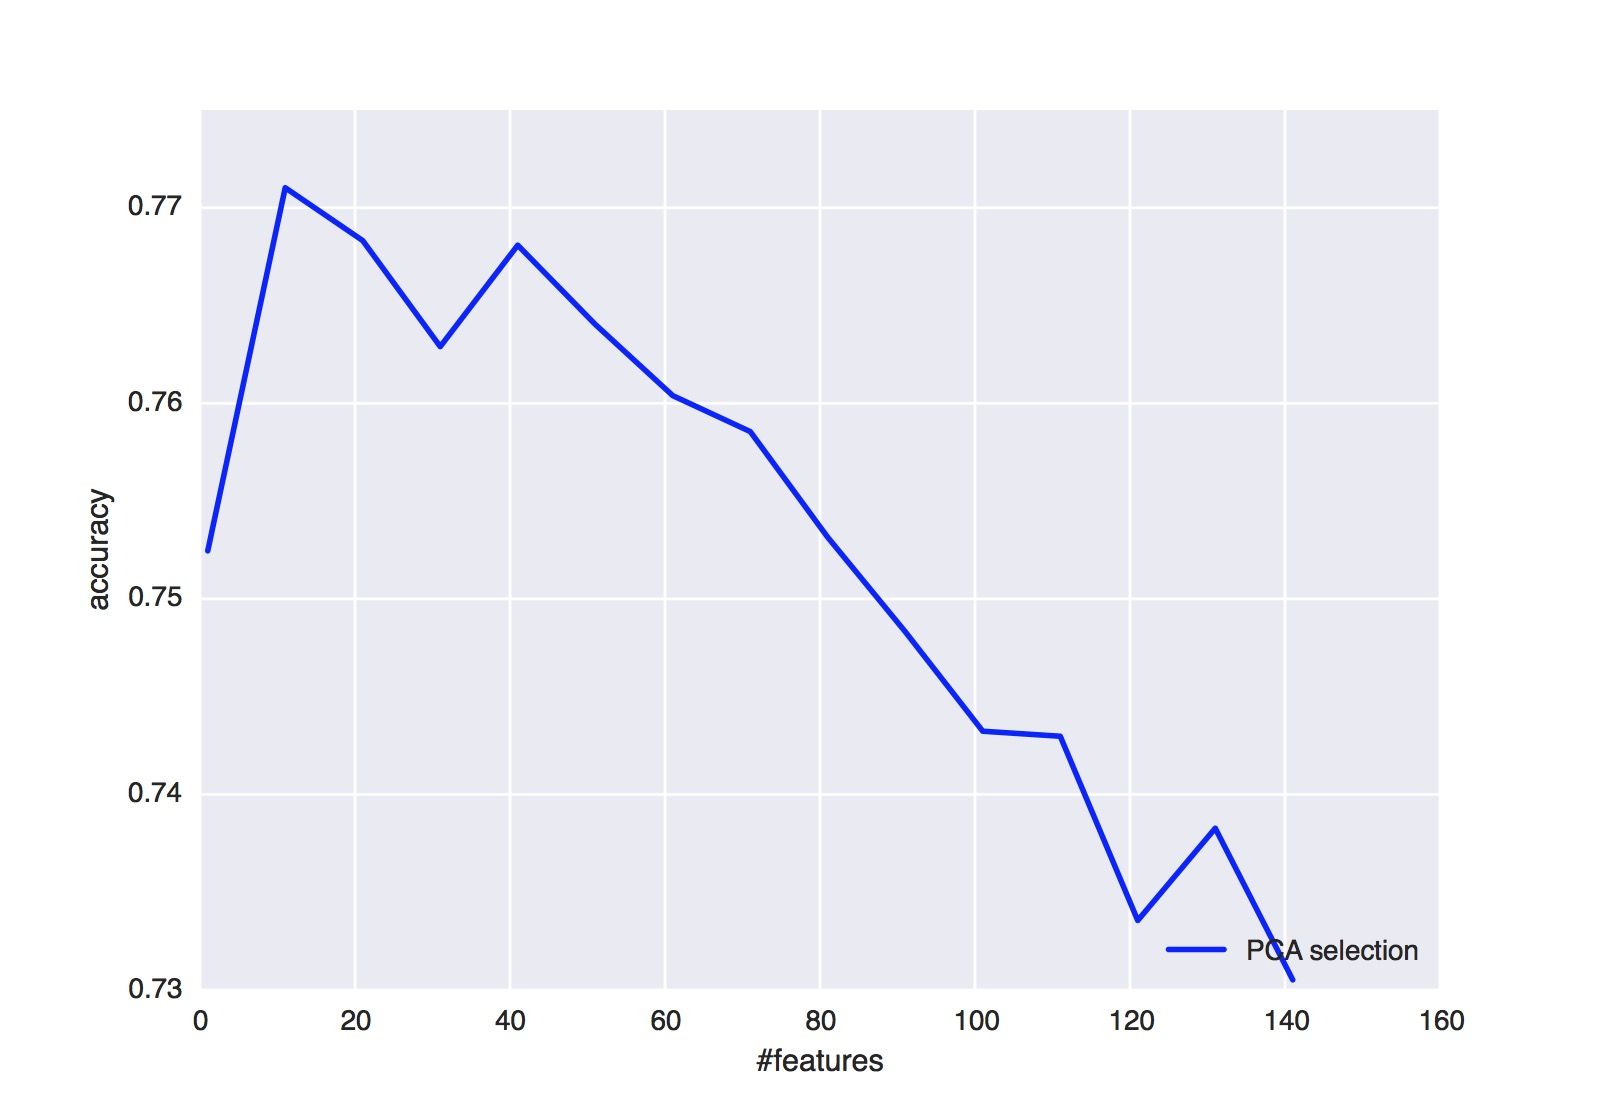
\includegraphics[scale=0.2]{figures/bernoulli_pca.jpg}
	\caption{Accuracy en función de cantidad de features resultante}
\end{figure}

El resultado en este caso es distinto. Si bien vemos que una cantidad de features insignificante (15/1000) logra un accuracy alto, se alcanza
un máximo rápidamente y luego la función comienza a decrecer con velocidad. Esto puede deberse a que el resto de las features aporten principalmente
ruido al modelo. Además, estimamos que decrece de manera logarítmica porque al ver la tabla de varianza explicada por componente que provee sklearn
se veía claramente que cada componente explicaba una potencia menos que la anterior aproximadamente.
